\documentclass[11pt]{article}

\usepackage{graphicx}
\usepackage[top=25mm, bottom=25mm, left=25mm, right=25mm, a4paper]{geometry}
\usepackage{amsmath}
\usepackage{mathrsfs}
\usepackage{enumitem}
\usepackage{float}
\usepackage{fancyhdr}
\usepackage{booktabs}
\usepackage{upquote}
\usepackage{tikz}
\usepackage{steinmetz}

\pagestyle{fancy}
\fancyhf{}
\fancyhead[R]{Baturay Kafkas - 2240357068 - Electrical \& Electronics Engineering}

\rfoot{\thepage}
\renewcommand{\headrulewidth}{0pt} 
\renewcommand{\footrulewidth}{0pt}
\sloppy

\begin{document}

\begin{center}
\large
\textbf{ELE228 - Programming for Circuits and Systems Preliminary Work 3}
\end{center}

\section{Questions}

\begin{enumerate}[leftmargin=*,label=\textbf{\arabic*.}]

\item Consider the circuit in \textit{Fig. 1}. Derive the numerical expression of the transfer function
\[H(s)=\frac{V_o(s)}{V_g(s)}.\]

\item Using MATLAB, find the numerical value of each pole and zero of $H(s)$ and plot the pole-zero map.

\item Evaluate the inverse Laplace transform of $H(s)$ to find the impulse response $h(t)$. Verify your result using MATLAB. Create a suitable time vector and plot $h(t)$ against time. Obtain the impulse response using the \texttt{impulse} command as well and compare the plots.

\item Using the transfer function $H(s)$, find the output voltage $V_o(s)$ when $V_g(s)$ is a unit step function. Evaluate the inverse Laplace transform of $V_o(s)$ to find $v_o(t)$. Verify your result using MATLAB. Create a suitable time vector and plot $v_o(t)$ against time. Obtain the step response using the \texttt{step} command as well and compare the plots.

\begin{figure}[h]
    \centering
    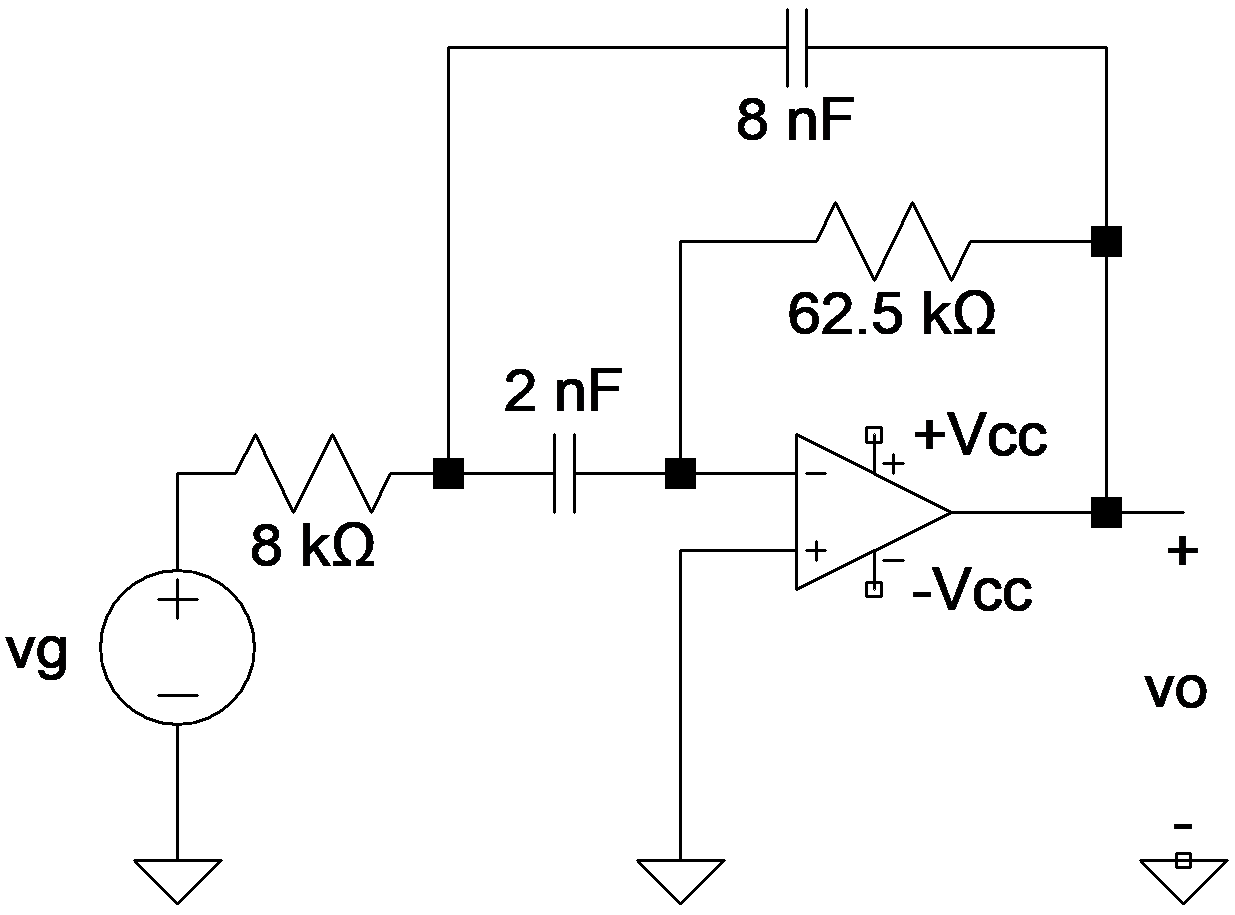
\includegraphics[width=0.5\linewidth]{cct1.png}

    \textit{Figure 1}
\end{figure}

\end{enumerate}

\section{Answers}

The $s$--domain equivalent circuit:

\begin{figure}[H]
    \centering
    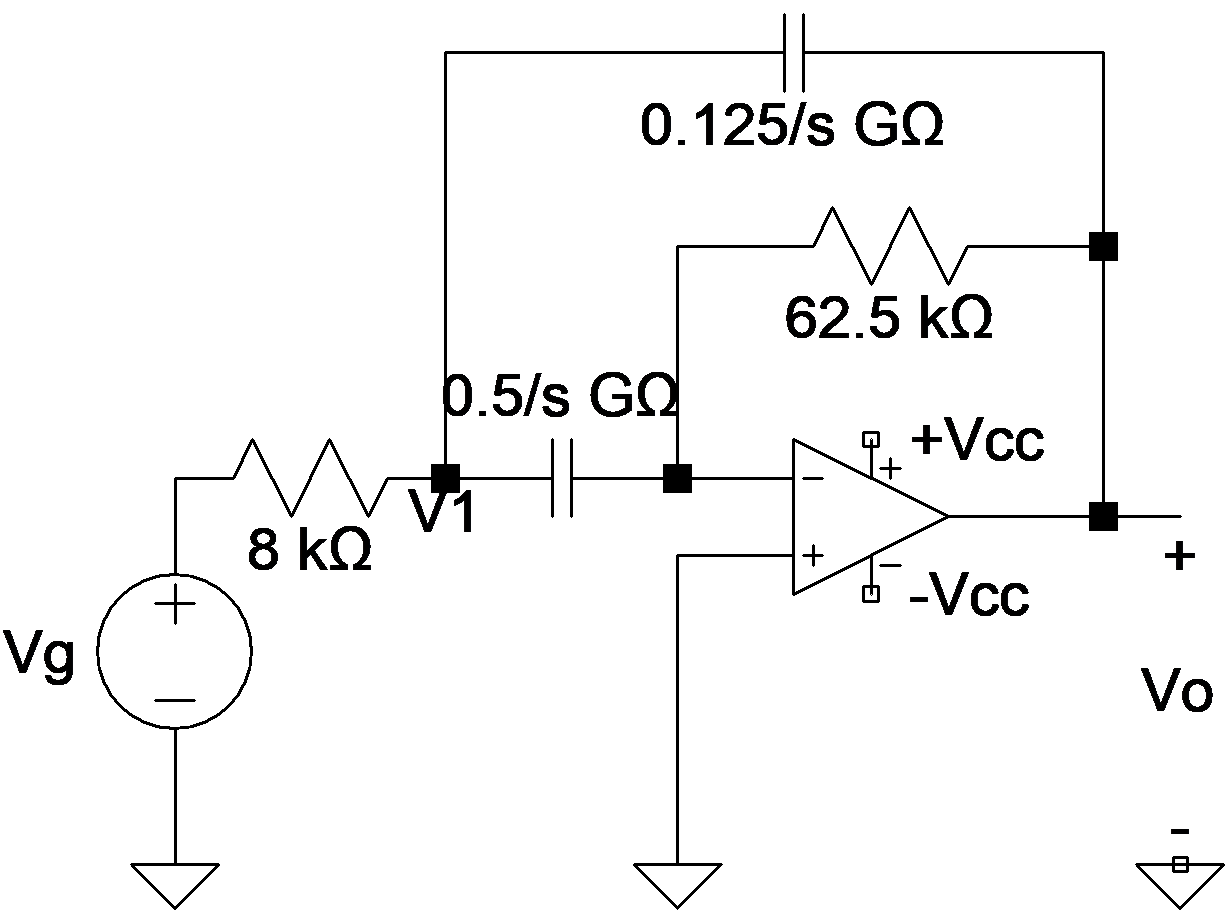
\includegraphics[width=0.5\linewidth]{cct2.png}

    \textit{Figure 2}
\end{figure}


\begin{enumerate}[leftmargin=*,label=\textbf{\arabic*.}]

\item KCL at node $V_1$:
\begin{equation}\frac{V_1-V_g}{8000}+\frac{sV_1}{5\cdot10^8}+\frac{(V_1-V_0)s}{0.125\cdot10^9}=0\implies(625\cdot10^2+5s)V_1-4sV_0=625\cdot10^2\cdot V_g\end{equation}

KCL at the negative terminal of the op--amp:
\begin{equation}\frac{(0-V_1)s}{5\cdot10^8}+\frac{0-V_o}{62500}=0\implies V_1=\frac{-8000}sV_o\end{equation}

Substitute $(2)$ into $(1)$:
\[(62500+5s)\frac{-8000}sV_o-4sV_o=62500V_g\implies\boxed{\frac{V_s}{V_g}=-\frac{15625s}{s^2+10000s+125\cdot10^6}}\]

\item Code:

\vspace{1em}

\hrule
\begin{verbatim}
num = [-15625 0];
denom = [1 10000 1.25e8];

H = tf(num, denom)
P = pole(H)
Z = zero(H)
pzmap(H)
\end{verbatim}
\hrule

\begin{figure}[H]
    \centering
    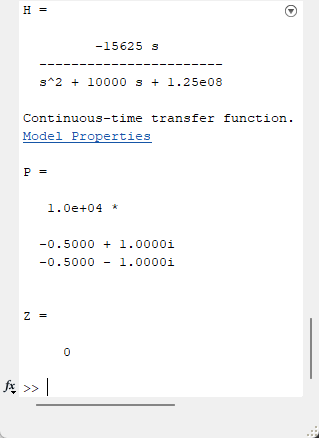
\includegraphics[width=0.5\linewidth]{MATLAB_ufF3HwZ57I.png}
\end{figure}

\begin{figure}[H]
    \centering
    
\includegraphics[width=0.55\linewidth]{q2.png}
\end{figure}

\item $h(t)$ is the inverse Laplace transform of $H(s)$.
\[H=\frac{-15625s}{s^2+10000s+1.25\cdot10^8}=\frac{-15625s}{(s+5000-j10000)(s+5000+j10000)}\]
\[H=\frac{K_1}{s+5000-j10000}+\frac{K_1^*}{s+5000+j10000}\]
\[K_1=H\cdot(s+5000-j10000)\bigg|_{s=-5000+j10000}=8734.64\phase{-153.43^\circ}\]
\[\implies \boxed{h(t)=[17469.28e^{-5000t}\cos(10000t-153.43^\circ)]u(t)}\]

Code:

\vspace{1em}

\hrule
\begin{verbatim}
syms s t;
H_sym = poly2sym(num, s) / poly2sym(denom, s);
h = ilaplace(H_sym)
time = [0:10^(-6):1.5*10^(-3)];
figure

subplot(2, 1, 1);
h_vals = subs(h, t, time);
plot(time, h_vals)
xlabel('Time (seconds)')
ylabel('Amplitude')
title('Impulse Response without the Impulse Command')

subplot(2, 1, 2);
impulse(H, time)
title('Impulse Response with the Impulse Command')
\end{verbatim}
\hrule

\begin{figure}[H]
    \centering
    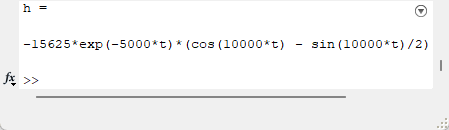
\includegraphics[width=0.5\linewidth]{MATLAB_pZ2TDqKYGj.png}
    
\includegraphics[width=0.5\linewidth]{q3.png}
\end{figure}

\item Obtain the Laplace transform of the unit step function.
\[\mathscr{L}\left\{u(t)\right\}=\frac1s=V_g\implies V_o(s)=\frac{-15625s}{s^2+10000s+0.125\cdot10^9}\]
\[V_o=\frac{K_1}{s+5000-j10000}+\frac{K_1^*}{s+5000+j10000}\]
\[K_1=V_o\cdot(s+5000-j10000)\bigg|_{s=-5000+j10000}=0.78\phase{90^\circ}\]
\[\implies \boxed{v_o(t)=[1.56e^{-5000t}\cos(10000t+90^\circ)]u(t)\text{ V}}\]

Code:

\vspace{1em}

\hrule
\begin{verbatim}
V_g = 1/s;
V_o = V_g * H_sym;
v_o = ilaplace(V_o)
figure

subplot(2, 1, 1);
v_o_vals = subs(v_o, t, time);
plot(time, v_o_vals)
xlabel('Time (seconds)')
ylabel('Amplitude')
title('Step Response without the Step Command')

subplot(2, 1, 2);
step(H, time)
title('Step Response with the Step Command')
\end{verbatim}
\hrule

\begin{figure}[H]
    \centering
    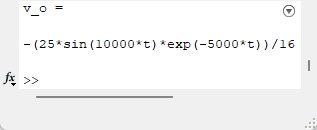
\includegraphics[width=0.4\linewidth]{MATLAB_DykvNop2fH.png}
    
\includegraphics[width=0.7\linewidth]{q4.png}
\end{figure}

\end{enumerate}

\end{document}